\chapter{Preliminaries and Related Work}

\section{Accounting Terminology}

Our terminology follows the accounting and auditing literature. A balance sheet consists of liabilities (value owed to others) and assets (value owned). When total asset value is the same or more than total liabilities, the firm is called solvent. The amount by which the assets exceed the liabilities is called capital or equity (depending on context). Some literature prefers the term `proof of reserves' to `proof of solvency.' This terminology is also sound, although it is not always defined correctly: technically a reserve is an asset that cancels out a corresponding liability, both in amount and in type. A firm can be solvent but not have full reserves. Most banks operate this way with cash liabilities, some assets in cash, but most assets in loans and other investments.\footnote{Banks in the United States have reserve requirements while banks elsewhere, \eg Canada, have capital requirements. Capital requirements speak to solvency, while reserve requirements speak to reserve ratios. Banks that underwent the 2008 financial crisis were more robust when they had capital requirements, as opposed to reserve requirements.} Cryptographic protocols in the literature generally assume both liabilities and assets are the same cryptocurrency so exchanges are expected to be both solvent and have full reserves.

\section{Related Work}
\label{sec:rw}

% !TEX root = ../main.tex

\begin{table}[t]
\centering
\begin{tabular}{|p{2.5cm}|p{7cm}|p{2.5cm}|}
\hline

$\Sigma$-Protocols 
& The first proofs of solvency are based on $\Sigma$-Protocols which work on standard elliptic curves like \secp but are not succinct (linear proof space, linear verifier time, heavy constants). 
& Provisions~\cite{provisions} \\ \hline

Inner-product arguments 
& Protocols like bulletproofs work on standard elliptic curves like \secp and can reduce some sub-routines (e.g., range arguments) to constant space and logarithmic verifier time. 
& Bulletproofs~\cite{bulletproofs} \\ \hline

Liabilities only 
& As it is the asset-side of solvency that ties the protocol to standard elliptic curves like \secp, proving only the liability side can be done in any cryptographic setting. 
& ZeroLedge~\cite{zeroledge}, DAPOL+~\cite{dapol}, SSVT-based~\cite{spp}, Notus~\cite{notus}, SafeCex\tablefootnote{V. Buterin, ``Having a safe CEX: proof of solvency and beyond,'' \href{https://web.archive.org/web/20230919210728/https://vitalik.ca/general/2022/11/19/proof_of_solvency.html}{vitalik.ca}, 2022} \\ \hline

Publish assets 
& A trivial proof of assets is one that is not zero-knowledge. An exchange could reveal all its addresses and prove ownership by signing a proof-specific message from each address.
& Summa\tablefootnote{\url{https://summa.gitbook.io/summa}} \\ \hline

Circuit-level 
& A general zk-snark can implement any arithmetic circuit, including \secp operations, which offers a proof of constant size and constant verifier time. 
& IZPR~\cite{izpr}, Proven.tools\tablefootnote{\url{https://www.proven.tools/}} \\ \hline

Custom blockchain 
& If new blockchains are deployed, they could use digital signatures over pairing-friendly curves. 
& Mina\tablefootnote{\url{https://minaprotocol.com/}} \\ \hline

Mapping between groups 
& If \secp values can be mapped to a pairing-friendly group, Poly-IOP arguments can potentially reduce the rest of the proof to constant size and constant verifier time. 
& COPZ~\cite{chase22}, \Sys \\ \hline

\end{tabular}
\caption{How to deal with the fact that Bitcoin and Ethereum use \secp digital signatures when trying to make a succinct proof of solvency.\label{tab:rb1}}
\end{table}

%\begin{figure}[t]
%\centering
%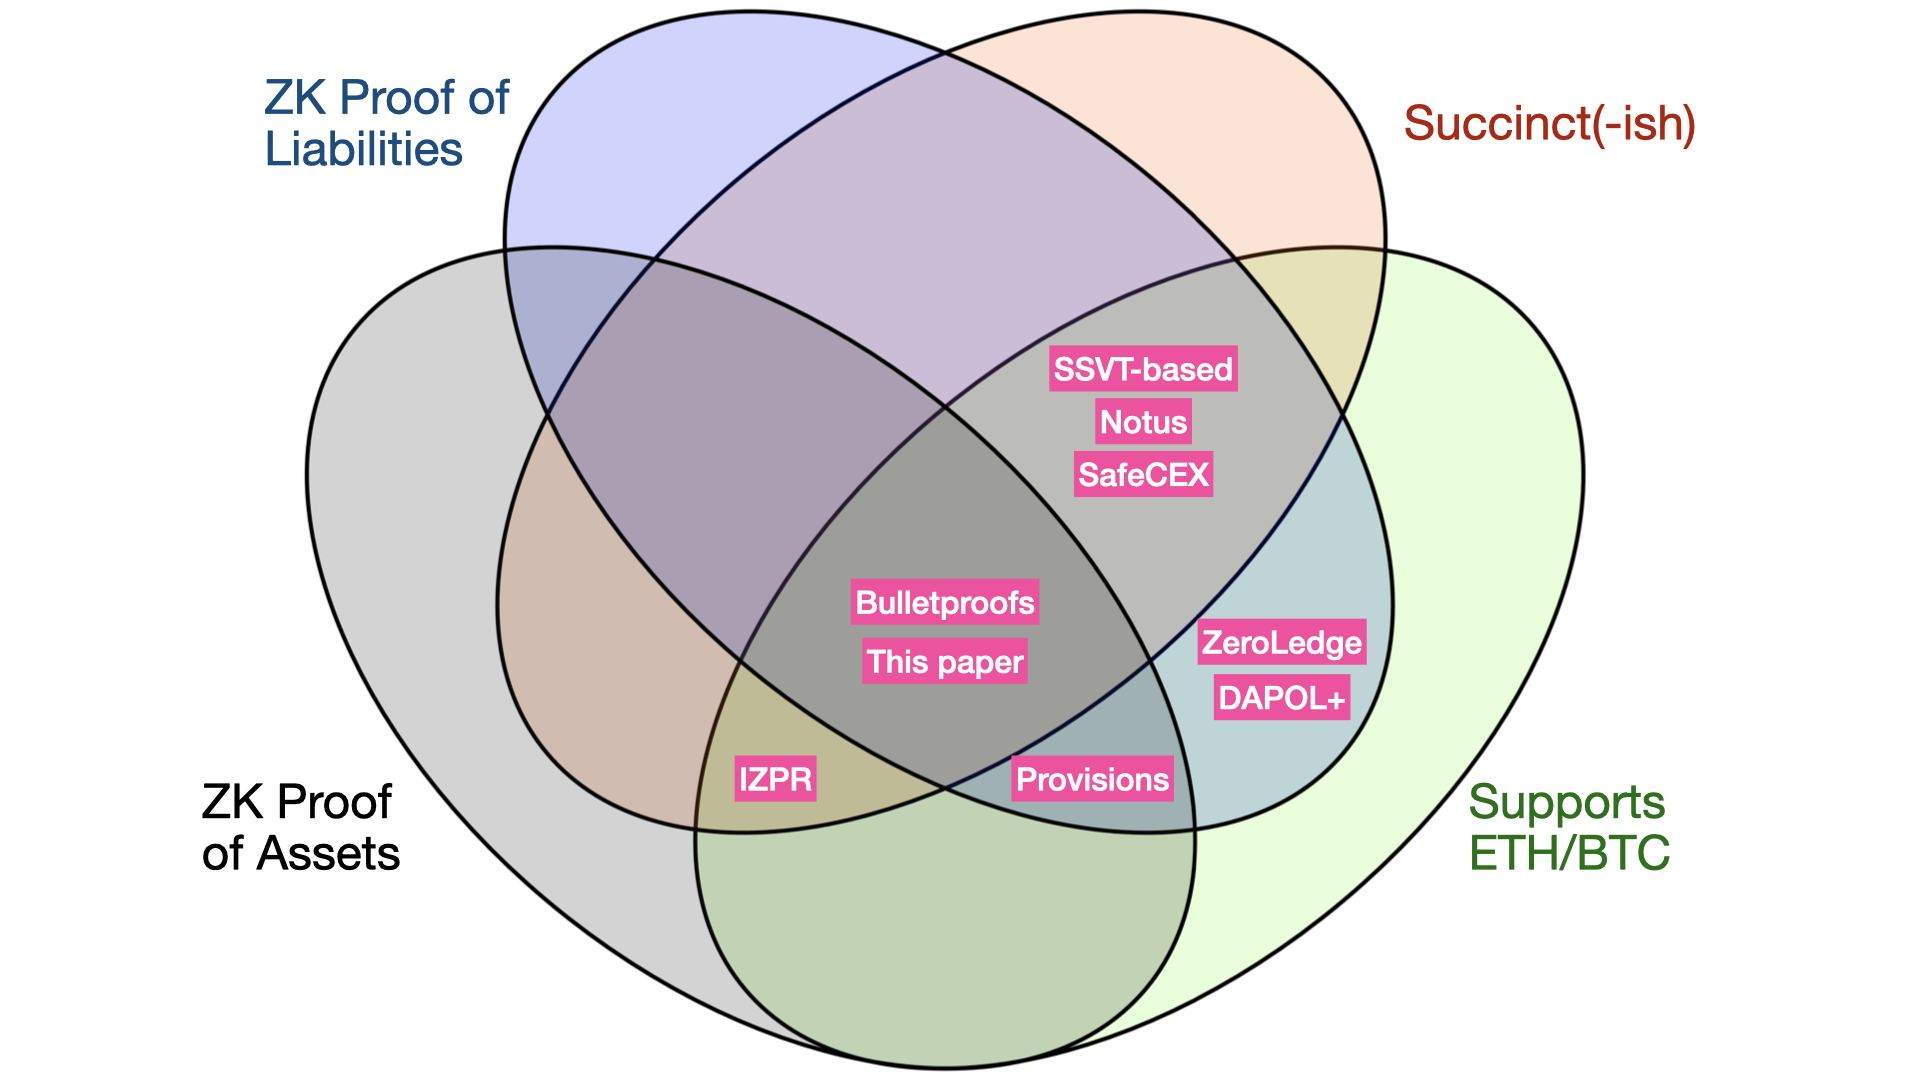
\includegraphics[width=0.8\textwidth]{figures/venn.png}
%\caption{default. \label{default}}
%\end{figure}

Proofs of solvency began as a discussion on Bitcointalk, where a protocol was developed for an exchange to announce a commitment to a total liability, and offer a Merkle-tree proof to each user that their balance was reflected in this total liability amount. Provisions, a research paper, used homomorphic commitments and $\Sigma$-protocols to add zero-knowledge, plus it added a proof of assets that could be used with the proof of liabilities to prove overall solvency~\cite{provisions}. As Provisions relies heavily on range proofs for liabilities, Bulletproofs can reduce the proof size of Provisions by 300x~\cite{bulletproofs}. Our protocol uses a polynomial-based range proof~\cite{rangeproof} to further reduce proof size and verifier time.

Outside of Provisions, Bulletproofs, and \Sys, the vast majority of work on proofs of solvency have not attempted an end-to-end proof, focusing instead on just the liabilities or just the assets. Why? We hypothesize that the biggest impediment is that Bitcoin and Ethereum assets are controlled by \secp private keys (see Table~\ref{tab:rb1}). Outside of Bulletproofs (based on inner-product arguments that do not require bilinear pairings and thus, can be implemented in \secp), most other approaches to succinctness require a specific cryptographic setting that is not \secp (\ie RSA for accumulators, pairing-based cryptography for zk-SNARKs, and lattices for zk-STARKs). If one only considers liabilities, then this problem does not have to be dealt with.

Circuit-based solutions are feasible but expensive for the prover---the authors of IZPR report about 500K constraints needed per key and proving times in the order of days for an anonymity set of 6000 keys~\cite{izpr}. By contrast, \Sys is a few minutes of work for the prover for 6000 keys. As this part is not-succinct (it is based on $\Sigma$-protocols), the trade-off is that the verifier has to do a few minutes of work as well. In both cases, IZPR and \Sys, this step does not need to be repeated often, only when the exchange wants to introduce new keys holding its assets. It is also important to recognize IZPR can let the exchange add keys it has not used yet to $\pi_{keys}$, further reducing how often this proof needs to be redone. This is a desirable property we are not able to easily achieve in \Sys (in short, it is due to our  use of selector polynomials instead of lookup arguments but future work could explore blending the best properties of \Sys and IZPR). 

% = = = = = = = = = = = = = = = = = = = = = = = = = = = = = = = = = = =

\section{Cryptographic Background}

We assume our protocol works in a finite field of prime order. For simplicity, we use $\prv$ and $\vrf$ to denote the prover and the verifier in an interactive proof system respectively. We use $g_\mathfrak{g}$ to denote a generator in a group $\mathbb{G}_\mathfrak{g}$ while $h_\mathfrak{g}$ is another generator, and no one knows the relative discrete logarithm of these two generators. Particularly, we use $\gs$ and $\hs$ to denote the two generators in $\mathbb{G}_s$, the \secp group; and we use $\gb$ and $\hb$ to denote the two generators in $\mathbb{G}_b$, the \bls group. If we need to distinguish which group an input to the pairing is from, we use the notations $[x]_1:=g_1^x,[x]_2:=g_2^x$, otherwise elements are  assumed to be in the first group (including $g_s$ and $g_b$). We use $e([x]_1,[x]_2)$ to denote a non-degenerate bilinear pairing. We use $\hash$ to denote a collision-resilient hash function modelled as a random oracle. We use $\ppt$ to represent probabilistic algorithms run in polynomial time.  For vectors, we use an overhead bar to denote a vector and brackets to denote the elements in this vector, e.g., $\overline{v}=\tuple{v_1,v_2,\dots}$. We also use a vector at the top right of a variable to indicate this variable belongs to this vector for readability, e.g., $x^{(\overline{v})}$ means $x$ is an element of $\overline{v}$. When we say the summation between two vectors $\overline{a},\overline{b}$, the result is a new vector $\overline{c}$ where each element is the summation of the elements from $\overline{a}$ and $\overline{b}$ at the same row.

\subsection{Discrete Logarithm Assumption}
\label{sec:dlp}
The discrete logarithm problem describes, given a triplet $(\mathbb{G}, p, g)$, where $\mathbb{G}$ is a cyclic group of order $p$ generated by $g\in\mathbb{G}$, and an element $y\in\mathbb{G}$, for a given adversary $\mathcal{A}$, $\mathcal{A}$ needs to compute an $x$ such that $y=g^x$. The discrete logarithm assumption holds for $\mathbb{G}$ if it is infeasible for $\mathcal{A}$ to find such $x$ in polynomial time.

\subsection{Pedersen Commitment}
\label{sec:pedersen}
The Pedersen commitment scheme \cite{pedersen} enables $\prv$ to \textit{commit} to a value $x$ without revealing it. Pedersen commitment provides perfectly hiding and computational binding based on the discrete logarithm assumption. Additionally, Pedersen commitments are \textit{additively homomorphic}: given two commitments $C_1$ and $C_2$, the summation of their secrets $x_1$ and $x_2$ is the secret of $C_1+C_2$. We use $\textbf{C}(x)$ to denote a Pedersen commitment to the value $x$. Particularly, we use $\ps$ to denote a Pedersen commitment in \secp and $\pb$ to denote a Pedersen commitment in \bls.

\subsection{Zero-Knowledge Proofs}
Informally, a zero-knowledge proof is a cryptographic protocol allowing $\prv$ to convince $\vrf$ that the claiming statement is true without revealing additional information, except the fact that the statement's truth. A zero-knowledge proof must satisfy the following properties:
\begin{enumerate}
    \item \textbf{Completeness:} If the statement is true, $\vrf$ will be convinced.
    \item \textbf{Soundness:} If the statement is false, the probability that $\vrf$ is convinced is negligible.
    \item \textbf{Zero-knowledge:} If the statement is true, $\vrf$ learns nothing except the fact that the statement is true.
\end{enumerate}

\subsection{$\Sigma$-Protocol}
\label{sec:sigma}
The $\Sigma-$protocol is a three-move interactive proof system. We define the $\Sigma-$protocol similarly to \cite{damgard10}. \\
\textbf{Definition 1.} \textit{Let $R$ be a binary relation between the statement $x$ and the witness $w$. Given common input $x$ to }$\prv$\textit{ and }$\vrf$\textit{, and private input $(x,w)$ such that $(x,w)\in{R}$ to }$\prv$\textit{, they run the following protocol:}
\begin{enumerate}
    \item $\prv$ \textit{computes a message $m$ from $(x,w)$ and sends $m$.}
    \item $\vrf$ \textit{sends a random challenge $c$.}
    \item $\prv$ \textit{replies with $z$.}
\end{enumerate}
\textit{At the end of the protocol }$\vrf$ \textit{has the data $(x,m,c,z)$}. \textit{He decides to output }\textbf{acc}\textit{ or }\textbf{rej}\textit{; such that}
\begin{itemize}
    \item \textbf{\textit{Completeness}:} \textit{A $\Sigma-$protocol is complete if} $\prv$ \textit{follows the protocol to generate the message $(m,c,z)$,} $\vrf$ \textit{always accepts.}
    \item \textbf{\textit{Special soundness}:} \textit{A $\Sigma-$protocol is special sound if there exists a $\ppt$ extractor $\mathcal{E}$, given any input $x$ and any two accepting $(m,c,z),(m,c^\prime,z^\prime)$ where $c\ne{c^\prime}$, $\mathcal{E}$ can compute $w$ where $(x,w)\in{R}$.}
    \item \textbf{\textit{Honest verifier zero-knowledge}:} \textit{A $\Sigma-$protocol is honest verifier zero-knowledge if there exists a $\ppt$ simulator $\mathcal{S}$, such that the transcript produced by $\mathcal{S}$ is indistinguishable from the messages between }$\prv$\textit{ and }$\vrf$\textit{.}
\end{itemize}
A commonly well-known way to convert a $\Sigma-$protocol into non-interactive is using the Fiat-Shamir transform \cite{fs}. But we still use the standard interactive $\Sigma-$protocol to demonstrate our work for comprehension.

\subsection{Disjunction of $\Sigma$-Protocols (OR Proof)}
The disjunction of $\Sigma$-protocols (OR proof) allows $\prv$ to prove the claimed $x$ is $x_1$ or $x_2$ through a $\Sigma$-protocol. Specifically, given two inputs $x_1,x_2$, $\prv$ proves he knows a $w$ such that $(x_1,w)\in{R_1}$ or $(x_2,w)\in{R_2}$, but $\vrf$ cannot learn which one $\prv$ knows. We use the same definition as \cite{damgard10}. \\
\textbf{Definition 2.} \textit{The OR proof is a $\Sigma-$protocol that given two inputs $x_1,x_2$,} $\prv$ and $\vrf$ \textit{run the following protocol:}
\begin{enumerate}
    \item $\prv$ \textit{computes the message $m_1$ using $(x_1,w)$ as input.} \\
    $\prv$ \textit{randomly generates $c_2$ as the challenge for $x_2$ and runs the simulator $\mathcal{S}(x_2,c_2)$ to produce $(m_2,z_2)$.}
    \item $\prv$ \textit{sends $m_1$ and $m_2$.}
    \item $\vrf$ \textit{sends a master challenge $c$.}
    \item $\prv$ \textit{computes $c_1=c\oplus{c_2}$ and $z_1$ on inputs $(x_1,c_1,m_1,w)$.} \\
    $\prv$ \textit{sends $(c_1,c_2,z_1,z_2)$.}
\end{enumerate}
\textit{At the end of the protocol} $\vrf$ \textit{verifies $c=c_1\oplus{c_2}$ and both $(m_1,c_1,z_2)$ and $(m_2,c_2,z_2)$ are valid to output} \textbf{acc} \textit{or} \textbf{rej}\textit{; such that}
\begin{itemize}
    \item \textit{\textbf{Completeness:} The case of $c_2$ is always accepted by} $\vrf$ \textit{as the definition of a simulator; on the other side, the case of $c_1$ has no difference from the standard $\Sigma-$protocol. Therefore, the OR proof is complete.}
    \item \textit{\textbf{Special soundness:} Let} $\prv$ \textit{execute the protocol twice. Two accepting transcripts} 
    \[ (x_1,x_2,c,c_1,c_2,z_1,z_2),(x_1,x_2,c^\prime,c_1^\prime,c_2^\prime,z_1^\prime,z_2^\prime),c\ne{c^\prime} \] 
    \textit{are given. It is clear that for some $s=1$ or $2$, the witness $w$ such that $(x_s,w)\in{R}$ can be extracted through an extractor $\mathcal{E}$ by the special soundness of $\Sigma$-protocol.}
    \item \textit{\textbf{Honest verifier zero-knowledge}: Given a master challenge $c$, choose $c_1$ or $c_2$ randomly and the other will be determined. Let the simulator run twice: $\mathcal{S}(x_1,c_1),\mathcal{S}(x_2,c_2)$. }
\end{itemize}
We use $x={x_1\orproof{x_2}}$ to denote $x$ is $x_1$ or $x_2$.

\subsection{Roots of Unity}
\label{app:rou}

\begin{figure}
\centering
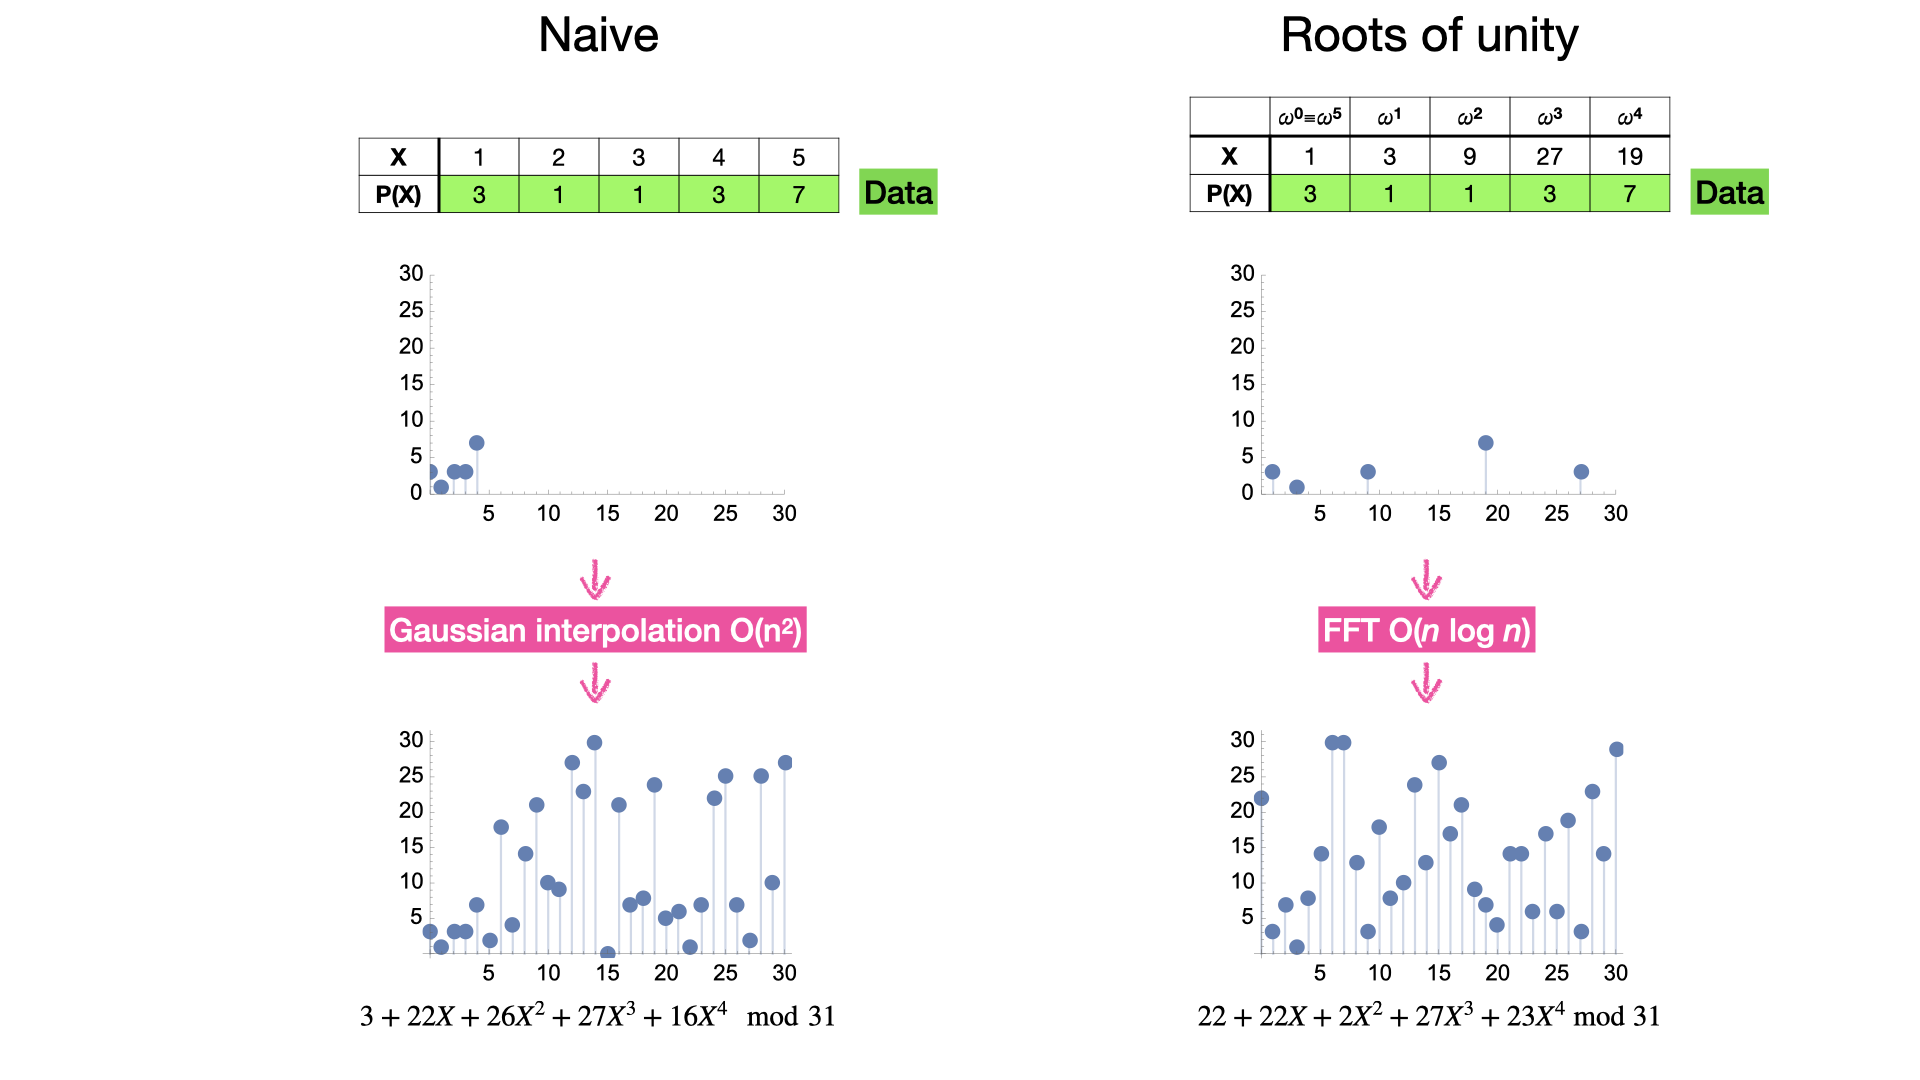
\includegraphics[width=\textwidth]{roots}
\caption{Small number ($\mathbb{Z}_{31}$) example of encoding a vector of integers $\tuple{3,1,1,3,7}$ into (a) the first 5 points of a polynomial, and (b) into 5th roots of unity ($\omega=3$).\label{fig:rou}}
\end{figure}

We use the approach of encoding data vectors into polynomials, committing to them using a polynomial commitment scheme (PCS), and forming zero knowledge arguments---a model called a polynomial-based interactive oracle proof (Poly-IOP). The zk-snark system Plonk popularized Poly-IOPs and has many extensions and optimizations. A one-dimensional vector of data is encoded into a univariate polynomial using 1 of 3 methods (all 3 are used at different steps of Plonk): (1) into the coefficients of the polynomial, (2) as roots of the polynomial, and (3) as the \(y\)-coordinates (\(\mathsf{data}_i=P(x_i)\)) of points on the polynomial. Plonk mostly relies on (3) and an interpolation algorithm is used to find the corresponding coefficients of the polynomial, which is
needed for the PCS. General interpolation algorithms are \(O(n^2)\) work for \(n\) evaluation points but this can be reduced to \(O(n\log n)\) with an optimization.

The optimization enables interpolation via the fast Fourier transform (FFT). It concerns how to choose the \(x\)-coordinates, which will serve as the index for accessing the data: evaluating \(P(X)\) at \(x_i\) will reveal \(\mathsf{data}_i\). First note, \(x\)-coordinates are from the exponent group (\(Z_q\)) and the choices exceed what is feasible to use (\(2^{255}\) values in \bls). Any subset can be used and interpolated. The optimization is to chose them with a mathematical structure. Specifically, instead an additive sequence (e.g., \(0,1,2,3,\ldots\)), we use a multiplicative sequence
\(1,\omega,\omega\cdot\omega,\omega\cdot\omega\cdot\omega,\ldots\) or equivalently: \(\omega^0,\omega^1,\omega^2,\ldots,\omega^{\kappa-1}\). Further, the sequence is closed under multiplication which means that next index after \(\omega^{\kappa-1}\) wraps back to the first index: \(\omega^{k-1} \cdot \omega = \omega^\kappa = \omega^0=1\) (this property is also useful in proving relationships between data in the vector and its neighbouring values).

For terminology, we say \(\omega\) is a generator with multiplicative order \(\kappa\) in \(Z_q\). This implies \(\omega^\kappa=1\). Rearranging, \(\omega=\sqrt[\kappa]{1}\). Thus we can equivalently describe \(\omega\) as a \(\kappa\)-th root of 1. Finally, as 1 is the unity element in \(Z_q\), \(\omega\) is commonly called a \(\kappa\)-th root of unity.

For practical purposes, \(\kappa\) represents the length of the longest vector of data we can use in our protocol. Where does \(\kappa\) come from? Different elements of \(Z_q\) will have different multiplicative orders but every order must be a divisor of \(q-1\). Thus \(\kappa\) is the largest divisor of the exact value of \(q\) used in an elliptic curve standard. The value of $q$ in \bls has \(\kappa=2^{32}\) (for terminology, this called a \(2\)-adicity of \(32\)).

\subsection{Polynomial Commitment Scheme}
A polynomial commitment scheme (PCS) allows $\prv$ to commit to a polynomial to convince $\vrf$ that claimed evaluations are of the committed polynomial \cite{kzg}. We define PCS based on \cite{kzg,plonk,bdfg}. \\
\textbf{Definition 3.} \textit{A polynomial commitment scheme consists of three moves:} \textbf{gen}\textit{,} \textbf{com}\textit{, and} \textbf{open} \textit{such that}
\begin{enumerate}
    \item \textbf{gen}$(d)$ \textit{is an algorithm that given a random number $\tau\in\mathbb{F}$ and a positive integer d, outputs a structured reference string (SRS)} \textbf{srs} \textit{such that} 
    \[ \textbf{srs}=([1]_1,[\tau]_1,\dots,[\tau^{d-1}]_1,[1]_2,[\tau]_2) \]
    \item \textbf{com}(\textit{f}, \textbf{srs}) \textit{outputs a commitment} $\cm$ \textit{to f, where f is a polynomial over $\mathbb{F}$ of degree smaller than d.}
    \item \textbf{open} \textit{is a protocol that} $\prv$ \textit{is given input f}, \textit{and} $\prv$ \textit{and} $\vrf$ are both given
    \begin{itemize}
        \item \textbf{srs}
        \item $\cm$ - \textit{the commitment to $f$}
        \item $a$ - \textit{an evaluation point of $f$}
        \item $b$ - \textit{the claimed evaluation of $f(a)$}
    \end{itemize}
    \textit{They run the protocol as follows:}
    \begin{enumerate}
        \item $\prv$ \textit{reveals the proof $\pi$ for the pair $(a,b)$ where}
        \[ \pi=[\frac{f(x)-b}{x-a}]_1 \]
        \item $\vrf$ \textit{outputs} \textbf{acc} \textit{if and only if}
        \[ e(\cm-[b]_1,[1]_2)=e(\pi,[\tau-a]_2) \]
    \end{enumerate}
\end{enumerate}
\begin{itemize}
    \item \textit{\textbf{Completeness}: It is clear that $\pi$ exists if and only if $f(a)=b$, which means $\vrf$ always accepts the proof if $\prv$ follows the protocol.}
    \item \textit{\textbf{Knowledge soundness in the algebraic group model}: For any algebraic adversary $\mathcal{A}$ in an interactive protocol of PCS, there exists a $\ppt$ extractor $\mathcal{E}$ given access to $\mathcal{A}$'s messages during the protocol, and $\mathcal{A}$ can win the following game with negligible probability:}
    \begin{enumerate}
        \item \textit{Given the inputs that} $\prv$ \textit{can access, $\mathcal{A}$ outputs} $\cm$.
        \item \textit{$\mathcal{E}$ outputs $f\in\mathbb{F}_{<d}[X]$ from $\mathcal{A}$'s output.}
        \item \textit{$\mathcal{A}$ generates $\pi$ and the evaluation $b^\prime$ at the evaluation point $a$.}
        \item \textit{$\mathcal{A}$ wins if}
        \begin{itemize}
            \item $\vrf$ \textit{accepts the proof at the end of the protocol.}
            \item $b^\prime\ne{b}$.
        \end{itemize}
    \end{enumerate}
\end{itemize}
Our work uses PCS with the root of unity. We use $\omega$ to denote the root of unity. We use $\cm_f$ to denote a commitment to $f$.

\subsection{Range Proof}
\label{sec:range}

A range proof enables $\prv$ to convince $\vrf$ a value $x$ is in a specified range, e.g., $[0,2^k)$, without revealing $x$. Zero-knowledge range proofs (ZKRPs) have three typical approaches: square decomposition, $n$-ary decomposition, and hash chains~\cite{zkrp}. We use the polynomial-based range proof from Boneh \etal~\cite{rangeproof}.
\begin{enumerate}
    \item \textit{Given input $x$, decompose $x$ to a vector of binary digits $\overline{z}=\tuple{z_1,z_2,\dots,z_k}$, so that $x=\sum_{i=0}^{k-1}2^i\cdot{z_i}$} 
    \item \textit{Construct a vector $\overline{x}=\tuple{x_1,x_2,\dots,x_k}$ such that}
    \begin{align*}
        x_1&=x \\
        x_k&=z_k \\
        x_i&=2x_{i+1}+z_i,i\in[1,k-1]
    \end{align*}
    \item \textit{Interpolate a polynomial $f$ from $\overline{x}$ over a finite field $H$ of order $n$ with elements $\omega^0,\omega^1,\omega^2,\ldots$ (see Appendix~\ref{app:rou})} 
    \item \textit{Prove the following polynomials are vanishing in $H$}
    \begin{align*}
        w_1&:=[f(X)-x]\cdot\frac{X^n-1}{X-\omega^0} \\
        w_2&:=f(X)\cdot[f(X)-1]\cdot\frac{X^n-1}{X-\omega^{n-1}} \\
        w_3&:=[f(X)-2\cdot{f(X\omega)}]\cdot[f(X)-2\cdot{f(X\omega)}-1]\cdot(X-\omega^{n-1})
    \end{align*}
    \begin{enumerate}
        \item $\prv$ \textit{sends the commitment to $f(X)$}
        \item $\vrf$ \textit{sends a random challenge $\gamma$}
        \item $\prv$ \textit{sends the commitment to $q(X)=w/(X^n-1)$, such that}
        \[ w=w_1+\gamma\cdot{w_2}+\gamma^2\cdot{w_3} \]
        \item $\vrf$ \textit{sends a random evaluation point $\zeta\in\mathbb{F}$}
        \item $\prv$ \textit{replies with $f(\zeta),f(\zeta\omega),q(\zeta)$}
        \item $\vrf$ \textit{checks}
        \begin{enumerate}
            \item $w(\zeta)=q(\zeta)\cdot(\zeta^n-1)$
            \item $f(\zeta),f(\zeta\omega),q(\zeta)$ \textit{are the correct evaluations}
        \end{enumerate}
    \end{enumerate}
\end{enumerate}

\subsection{Batched opening with zero-knowledge extension ($\open$)}
\label{sec:kgzzkp}


To efficiently prove several polynomials are vanishing at several points, there are some batched KZG opening schemes such as the schemes in \cite{plonk,bdfg,fflonk}. Although a PCS does not reveal the committed polynomial directly, it leaks the information of the opening evaluation point. In our scenario, each evaluation is privacy-sensitive so we want to hide the polynomial evaluations. We use the opening scheme from \cite{plonk} and the protocol from \cite{rangeproof} with a zero-knowledge extension to explain how to prove the range-proof polynomials are vanishing efficiently and in zero-knowledge. \\
\textit{Assume $\prv$ is given $x$ and $\vrf$ is given $[x]_1$, $\prv$ wants to prove $x$ is in $[0,2^k)$:}
\begin{enumerate}
    \item $\prv$ \textit{interpolates the polynomial $f$ using the above range proof}
    \item $\prv$ \textit{generates two random numbers $\omega^{\prime},\omega^{\prime\prime}$ in $\mathbb{F}\setminus{H}$ and another two random numbers $\alpha,\beta$ in $\mathbb{F}$}
    \item $\prv$ \textit{interpolates $f^\prime$ at two more points ${\omega^{\prime},\omega^{\prime\prime}}$ such that}
    \[ f^\prime(\omega^{\prime})=\alpha \]
    \[ f^\prime(\omega^{\prime\prime})=\beta \]
    \item $\prv$ \textit{computes $w_1,w_2,$ and $w_3$ in the above range proof and sends the commitment to $f^\prime$,} $\cm_{f^\prime}$
    \item $\vrf$ \textit{sends a random challenge $\gamma\in\mathbb{F}$}
    \item $\prv$ \textit{sends the commitment to $q_w:=w/(X^n-1)$ where}
    \[ w:=w_1+\gamma\cdot{w_2}+\gamma^2\cdot{w_3} \]
    \item $\vrf$ \textit{sends a random evaluation point $\zeta\in\mathbb{F}\setminus{H}$}
    \item $\prv$ \textit{sends the evaluations $f(\zeta),f(\zeta\omega),q_w(\zeta)$}
    \item $\prv$ \textit{sends the commitments to $q_1(X),q_2(X)$, where}
    \[ q_1(X):=\frac{f(X)-f(\zeta)}{X-\zeta}+\gamma\cdot\frac{q_w(X)-q_w(\zeta)}{X-\zeta} \]
    \[ q_2(X):=\frac{f(X)-f(\zeta\omega)}{X-\zeta\omega} \]
    \item $\vrf$ \textit{chooses random $r\in\mathbb{F}$}
    \item $\vrf$ \textit{accepts the proof if and only if}
    \begin{enumerate}
    	\item $w_1(\zeta)+\gamma\cdot{w_2(\zeta)}+\gamma^2\cdot{w_3(\zeta)}=q_w(\zeta)\cdot(\zeta^n-1)$
    	\item $e(F+\zeta\cdot\cm_{q_1}+r\zeta\cdot\cm_{q_2},[1]_2)=e(\cm_{q_1}+r\cdot\cm_{q_2},[x]_2)$\textit{, where}
    	\begin{align*}
    		F:=&\cm_f-[f(\zeta)]_1+\gamma\cdot(\cm_{q_w}-[q_w(\zeta)]_1)da+r\cdot(\cm_f-[f(\zeta\omega)]_1)
    	\end{align*}
    \end{enumerate}
%    \item $\prv$ \textit{interpolates a polynomial $g$ such that $g(\tau)=f(\tau),g(\tau\omega)=f(\tau\omega)$ and sends $g$}
%    \item $\prv$ \textit{sends the commitment to $q_{w^\prime}:=w^\prime/(X^n-1)$, where}
%    \begin{align*}
%    	w^\prime:=&(f(X)-g(X))\cdot\frac{X^n-1}{(X-\tau)(X-\tau\omega)}
%    \end{align*}
%    \item $\vrf$ \textit{sends another random evaluation point $\rho\in\mathbb{F}$}
%    \item $\prv$ \textit{sends the commitment to $q_{\hat{w}}:=\hat{w}/(x-\rho)$, where}
%    \begin{align*}
%    	\hat{w}:=&(f(X)-g(\rho))\cdot\frac{\rho^n-1}{(\rho-\tau)(\rho-\tau\omega)}-q_{w^\prime}(X)\cdot(\rho^n-1)
%    \end{align*}
%    \textit{Note $\hat{w}$ is a zero polynomial for all $x\in\mathbb{F}$, which means $X-\rho$ divides $\hat{w}$}
%    \item $\vrf$ \textit{accepts the proof if and only if}
%    	\begin{enumerate}
%    		\item $w_1(\tau)+\gamma\cdot{w_2(\tau)}+\gamma^2\cdot{w_3(\tau)}=q_w(\tau)\cdot(\tau^n-1)$
%    		\item $g(\tau)=f(\tau),g(\tau\omega)=f(\tau\omega)$
%    		\item \textit{$e(F,[1]_2)=e([q_{\hat{w}}]_1,[x-\rho]_2)$, where}
%	    		\begin{align*}
%	    		F:=&(\cm_f-[g(\rho)]_1)\cdot\frac{\rho^n-1}{(\rho-\tau)(\rho-\tau\omega)}-[q_{\hat{w}}]_1\cdot(\rho^n-1)
%	    		\end{align*}
%    	\end{enumerate}
\end{enumerate}

We prove the protocol has zero knowledge. \\
\textit{Let $\mathcal{S}$ generate $\{\omega_i^\prime,\omega_i^{\prime\prime},\alpha_i,\beta_i\},i\in[0,m]$ and interpolate $\{f_i\}$ such that}
\[ f_i(\omega_i^\prime)=\alpha_i \]
\[ f_i(\omega_i^{\prime\prime})=\beta_i \]
\[ f_i(\omega^i)=0 \]
\textit{where $i\in[0,m]$ and $\omega$ is the root of unity in $H$. Note} $\vrf$ \textit{can interact with $\mathcal{S}$ to execute the protocol and accept the proof from $\mathcal{S}$. Given $\{\omega_i^\prime,\omega_i^{\prime\prime},\alpha_i,\beta_i\}_{i\in[0,m]}$ are chosen uniformly at random each time,} $\vrf$ \textit{cannot distinguish between the transcript from $\mathcal{S}$ and the proof from} $\prv$. \textit{Therefore, the protocol has zero knowledge. We will use} $\open$ \textit{to denote this opening technique.}

% = = = = = = = = = = = = = = = = = = = = = = = = = = = = = = = = = = =